\begin{frame}
	\frametitle{Motivation}
  
	\begin{itemize}
  		\item Why should I care about \emph{fingerprinting}?
    	\item How does it \emph{affect me}?
    	\item \emph{What can I do} to prevent it?
  	\end{itemize}
  
  	\bigskip

  	
\includegraphics[width=\textwidth]{img/tesla_ad.pdf}
\end{frame}

\begin{frame}
	\frametitle{Fingerprinting and inconsistencies}
	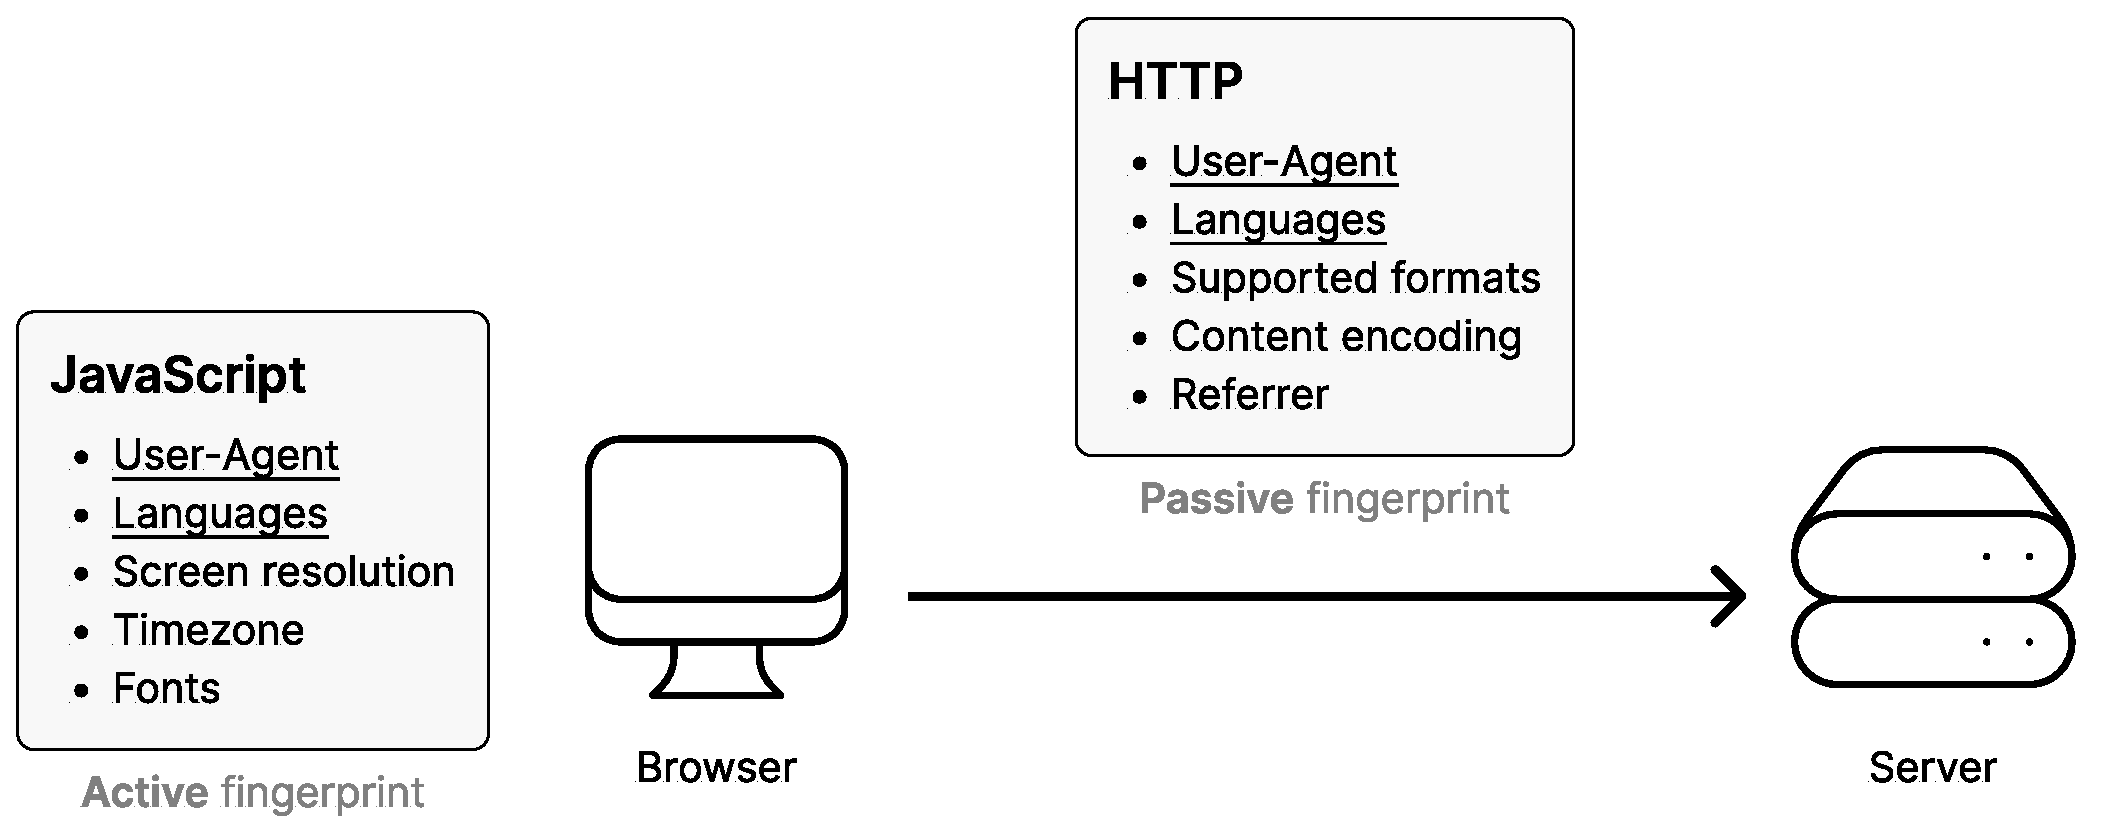
\includegraphics[width=\textwidth]{img/schema.pdf}
  
	\bigskip
  
	\begin{itemize}
		\item The fingerprinting application (Server) collects data from the device (Browser) \emph{actively} and \emph{passively}.
		\item \emph{Countermeasures} alter data to confuse the fingerprinter.
		\item When changed improperly, the fingerprinter can detect \underline{inconsistencies}.
	\end{itemize}
\end{frame}

\begin{frame}
	\frametitle{Active fingerprinting protection (JShelter)}
	
	\begin{columns}
		\column{0.6\textwidth}
		\begin{itemize}
			\item \emph{JShelter} is an anti-malware browser extension.
			\item Includes \emph{active} fingerprinting countermeasures.
			\item Lacks \emph{passive} fingerprinting countermeasures.
		\end{itemize}
		
		\column{0.4\textwidth}
			
\includegraphics[width=\textwidth]{img/jshelter-hero.pdf}
	\end{columns}
	
	\bigskip
	\bigskip
	
	My master thesis aims to design and implement passive fingerprinting protection to \emph{complement} the already existing protections of JShelter.
\end{frame}

\begin{frame}
	\frametitle{Minimizing user side effects}
	
	\emph{Description}:
	
	\begin{itemize}
		\item Every modification made to HTTP headers could result in a different response from the server.
		\item \emph{The goal} is to minimize these side effects, which could negatively affect the user experience.
	\end{itemize}
	
	\medskip
	
	\emph{Example:}
	
	\begin{itemize}
		\item English is a prevalent language on the web.
		\item Let's change the preferred language to English to create a \uv{homogenous} fingerprint.
		\item The site language changes to English, but the user doesn't understand English.
	\end{itemize}
\end{frame}

\begin{frame}
	\frametitle{HTTP Header: User-Agent}
	
	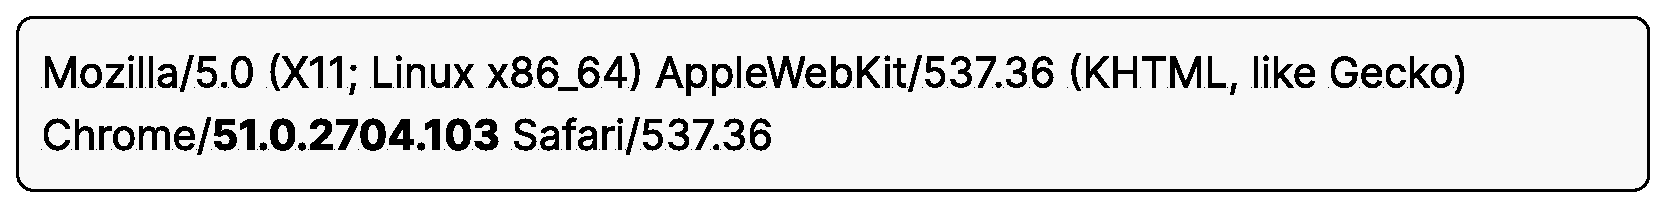
\includegraphics[width=\textwidth]{img/user-agent-1.pdf}

	\medskip
	
	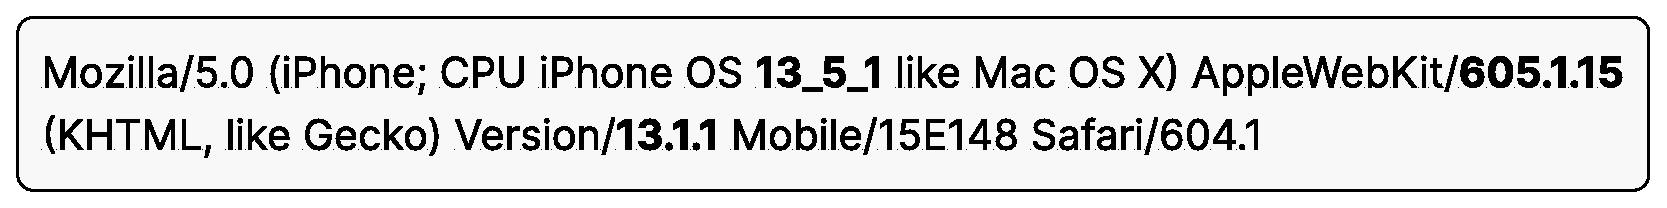
\includegraphics[width=\textwidth]{img/user-agent-2.pdf}
	
	\medskip
	
	\emph{Transformation:}
	
	\begin{itemize}
		\item \emph{Downgrade of version numbers} in the User-Agent string.
		\item Two version numbers that differ in the last segment (\emph{PATCH}) should have the same functionality (Semantic Versioning).
		\item \underline{Example:} \texttt{AWK/605.1.15} $\rightarrow$ \texttt{AWK/605.1.14}
	\end{itemize}
	
	\medskip
	
	\emph{Consistency:}
	
	\begin{itemize}
		\item An identical 1:1 copy stored in \texttt{Navigator.userAgent}.
	\end{itemize}
\end{frame}

\begin{frame}
	\frametitle{HTTP Header: Accept}
	
	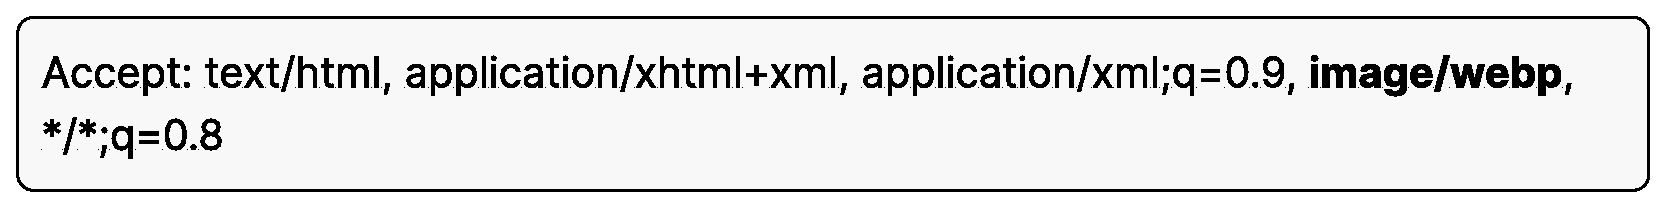
\includegraphics[width=\textwidth]{img/accept.pdf}
	
	\bigskip
	
	\emph{Transformation:}
	
	\begin{itemize}
		\item Replace newer formats with older alternatives.
		\item Would result in a performance hit, but not break the page.
		\item \underline{Example:} \texttt{image/webp} $\rightarrow$ \texttt{image/png}
	\end{itemize}
	
	\medskip
	
	\emph{Consistency:}
	
	\begin{itemize}
		\item It is not easy to detect inconsistencies as there is no interface listing all supported formats.
		\item The \texttt{Navigator.mimeTypes} interface that partially allowed this is deprecated.
	\end{itemize}
\end{frame}

\begin{frame}
	\frametitle{HTTP Header: Accept-Language}
	
	
\includegraphics[width=\textwidth]{img/accept-language.pdf}
	
	\bigskip
	
	\emph{Transformation:}
	
	\begin{itemize}
		\item Add, modify or remove \emph{language regions} (subtags).
		\item \underline{Example:}
			\begin{itemize}
				\item \texttt{en} $\rightarrow$ \texttt{en-GB}
				\item \texttt{fr-CH} $\rightarrow$ \texttt{fr-CA}
				\item \texttt{de-AT} $\rightarrow$ \texttt{de}
			\end{itemize}
	\end{itemize}
	
	\medskip
	
	\emph{Consistency:}
	
	\begin{itemize}
		\item Preferred languages are also available through the \texttt{Navigator.languages} interface.
		\item The first language is accessible through the \texttt{Navigator.language} interface.
	\end{itemize}
\end{frame}

\begin{frame}
	\frametitle{List of HTTP headers}
	
	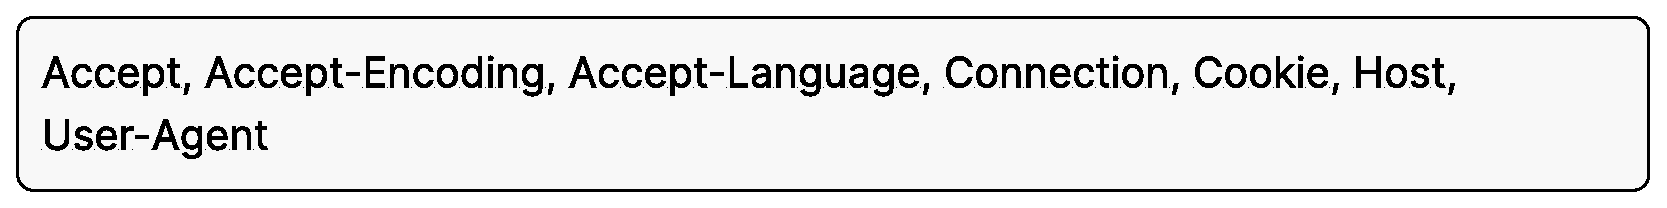
\includegraphics[width=\textwidth]{img/http-headers.pdf}
	
	\bigskip
	
	\emph{Transformation:}
	
	\begin{itemize}
		\item Add new headers to the HTTP request.
		\item Custom headers pose a low risk of a breaking event.
	\end{itemize}
	
	\medskip
	
	\emph{Consistency:}
	
	\begin{itemize}
		\item Not available through the browser APIs.
	\end{itemize}
\end{frame}

\begin{frame}
	\frametitle{The end}
	
	
\includegraphics[width=0.4\textwidth]{img/fitlogo1.pdf}
	
	\bigskip
	\bigskip

	\begin{huge}
		\emph{Thank you for your attention.}
	\end{huge}

	\medskip

	Jozef Hruška
\end{frame}